\documentclass[11pt,a4paper]{article}

\usepackage[utf8]{inputenc}
\usepackage[T1]{fontenc}
\usepackage{amsmath}
\usepackage{amsfonts}
\usepackage{amssymb}
\usepackage{graphicx}
\usepackage[colorlinks=true, citecolor=red, linkcolor=blue, urlcolor=blue]{hyperref}
\usepackage{booktabs}
\usepackage{listings}
\usepackage{xcolor}
\usepackage[margin=1in]{geometry}
\usepackage{physics}

% Code listing style
\lstdefinestyle{mystyle}{
    backgroundcolor=\color{gray!10},   
    commentstyle=\color{green!50!black},
    keywordstyle=\color{blue},
    numberstyle=\tiny\color{gray},
    stringstyle=\color{magenta},
    basicstyle=\ttfamily\footnotesize,
    breakatwhitespace=false,         
    breaklines=true,                 
    captionpos=b,                    
    keepspaces=true,                 
    numbers=left,                    
    numbersep=5pt,                  
    showspaces=false,                
    showstringspaces=false,
    showtabs=false,                  
    tabsize=2
}
\lstset{style=mystyle}

\title{Qubit Encoding and the Signatures of Majorana Modes}
\author{Jaskaran Singh, 3779140}
\date{\today}

\begin{document}

\maketitle

\section{Introduction}

The primary motivation for mapping fermionic systems to qubit models is the prospect of simulating complex quantum phenomena, such as the Kitaev chain, on quantum computers \cite{Kitaev2001}. Quantum hardware natively operates on two-level systems, or qubits, rather than fermions. This presents a fundamental mathematical challenge when attempting to simulate fermionic Hamiltonians directly. 

The core of this challenge lies in the fundamental algebraic properties of the particles involved. Fermions obey anticommutation relations. If we consider fermionic creation ($c_j^\dagger$) and annihilation ($c_i$) operators acting on sites $i$ and $j$, they satisfy the standard relation:
\begin{equation}
    \{c_i, c_j^\dagger\} = \delta_{ij}, \quad \{c_i, c_j\} = 0
\end{equation}
Conversely, quantum operators acting on distinct qubits commute with one another. Let $\sigma_j^\alpha$ denote the standard Pauli operators (where $\alpha \in \{x, y, z\}$) acting on qubit $j$. For different sites ($i \neq j$), the commutator is zero:
\begin{equation}
    [\sigma_i^\alpha, \sigma_j^\beta] = 0 \quad \text{for } i \neq j
\end{equation}
To successfully simulate the Kitaev chain, we must find a mathematical encoding that allows commuting qubit operations to emulate the anticommuting behavior of fermions \cite{Kitaev2001}.

\section{The Jordan-Wigner Transformation}

The standard technique to bridge the gap between fermionic and spin (qubit) algebras in one-dimensional systems is the Jordan-Wigner transformation \cite{JordanWigner1928}. This mapping achieves the required anticommutation by attaching a non-local "string" of Pauli $Z$ operators to each local fermionic operator. 

Physically, this Z-string acts as a parity counter for the preceding sites in the chain \cite{JordanWigner1928}. It encodes the fermion occupancy of all sites to the left of the target site, restoring the correct anticommutation relations when evaluating operators acting on different sites. Specifically, the transformation relates the fermionic annihilation and creation operators to the local qubit raising and lowering operators, $\sigma^\pm = \frac{1}{2}(X \pm iY)$, via:
\begin{equation}
    c_j = \left(\prod_{k=0}^{j-1}Z_k\right)\sigma_j^- 
\end{equation}
\begin{equation}
    c_j^\dagger = \left(\prod_{k=0}^{j-1}Z_k\right)\sigma_j^+
\end{equation}
To see why this string is necessary, consider the product of a creation operator at site $i$ and an annihilation operator at site $j$, where $i < j$. The Z-operators at sites $k \le i$ will evaluate to the identity or commute cleanly, but the remaining operators $Z_{i}\cdots Z_{j-1}$ from the string attached to $c_j$ remain. Because the local Pauli $Z_k$ operator flips sign when site $k$ is occupied, this string effectively tracks the parity of the intervening fermions, transforming the commutators of the qubit Hilbert space into the required anticommutators of the fermionic Hilbert space.

Using the standard properties of the Pauli matrices ($X^2=Y^2=Z^2=I$, and their anticommutation relations $\{X, Y\} = 0$), we can derive essential operator identities that will be used to map the Hamiltonian. The most fundamental is the number operator:
\begin{equation}
    c_j^\dagger c_j = \sigma_j^+ \sigma_j^- = \left(\frac{X_j + iY_j}{2}\right)\left(\frac{X_j - iY_j}{2}\right) = \frac{I - Z_j}{2}
\end{equation}
This identity demonstrates that the presence or absence of a fermion at site $j$ maps directly to the state of the qubit in the computational $Z$ basis \cite{JordanWigner1928}.

\section{Deriving the Qubit Hamiltonian}

With the operator mappings established, we can transform the fermionic Kitaev Hamiltonian into its qubit equivalent \cite{Kitaev2001}. We consider the Kitaev Hamiltonian with open boundary conditions:
\begin{equation}
    H_K = -\mu \sum_{j=0}^{L-1} c_j^\dagger c_j - t \sum_{j=0}^{L-2} (c_j^\dagger c_{j+1} + h.c.) + \Delta \sum_{j=0}^{L-2} (c_j^\dagger c_{j+1}^\dagger + h.c.)
\end{equation}
We proceed by applying the Jordan-Wigner transformation term by term.

\subsection{Chemical Potential Term}
Using the number operator identity derived above, the chemical potential maps directly to the single-qubit $Z$ basis. Dropping the constant energy offset $I/2$, this term manifests as a transverse magnetic field:
\begin{equation}
    -\mu \sum_{j} c_j^\dagger c_j = -\frac{\mu}{2} \sum_{j} (I - Z_j) \cong \frac{\mu}{2} \sum_{j} Z_j
\end{equation}
Depending on the sign convention (mapping the empty fermionic state to $\ket{0}$ where $Z=+1$), this is commonly written in the literature and simulation code as $-\frac{\mu}{2} \sum_j Z_j$.

\subsection{Hopping Term}
For the nearest-neighbor hopping term $c_j^\dagger c_{j+1}$, the product of operators causes the $Z$-strings to partially cancel. The term evaluates to:
\begin{equation}
    c_j^\dagger c_{j+1} = \left(\prod_{k=0}^{j-1}Z_k\right)\sigma_j^+ \cdot \left(\prod_{m=0}^{j}Z_m\right)\sigma_{j+1}^- = \sigma_j^+ Z_j \sigma_{j+1}^-
\end{equation}
Using the identity $Z_j = I - 2\sigma_j^+ \sigma_j^-$, we have:
\begin{equation}
    \sigma_j^+ (I - 2\sigma_j^+\sigma_j^-)\sigma_{j+1}^- = -\sigma_j^+\sigma_{j+1}^-
\end{equation}
Adding the Hermitian conjugate, we obtain:
\begin{equation}
    c_j^\dagger c_{j+1} + h.c. = -(\sigma_j^+\sigma_{j+1}^- + \sigma_j^-\sigma_{j+1}^+) = -\frac{X_j X_{j+1} + Y_j Y_{j+1}}{2}
\end{equation}
Multiplied by the hopping amplitude $t$, this term generates symmetric $XX$ and $YY$ couplings.

\subsection{Pairing Term}
Similarly, the superconducting pairing term maps to:
\begin{equation}
    c_j^\dagger c_{j+1}^\dagger = \sigma_j^+ Z_j \sigma_{j+1}^+ = -\sigma_j^+\sigma_{j+1}^+
\end{equation}
Adding its Hermitian conjugate yields:
\begin{equation}
    c_j^\dagger c_{j+1}^\dagger + h.c. = -(\sigma_j^+\sigma_{j+1}^+ + \sigma_j^-\sigma_{j+1}^-) = -\frac{X_j X_{j+1} - Y_j Y_{j+1}}{2}
\end{equation}
Multiplied by $\Delta$, this generates an asymmetric $XX$ and $YY$ coupling.

\subsection{Full Qubit Hamiltonian}
Combining all transformed terms, the fermionic Kitaev chain is rigorously mapped to a one-dimensional transverse-field $XY$ spin model \cite{JordanWigner1928, Kitaev2001}:
\begin{equation}
    H = -\frac{\mu}{2} \sum_{j} Z_j + \frac{t-\Delta}{2} \sum_{j} X_j X_{j+1} + \frac{t+\Delta}{2} \sum_{j} Y_j Y_{j+1}
\end{equation}

\section{The "Sweet Spot" and the AFM Ising Comparison}

The connection between topological phases and classical spin models becomes explicit at the "sweet spot" deep within the topological phase, defined by $t = \Delta$ and $\mu = 0$. Here, the $X_j X_{j+1}$ terms perfectly cancel out, and the transverse field vanishes, simplifying the Hamiltonian to:
\begin{equation}
    H_{\text{sweet}} = t \sum_{j} Y_j Y_{j+1}
\end{equation}
Algebraically, this possesses the exact same mathematical structure as a classical nearest-neighbor antiferromagnetic (AFM) Ising chain, written natively in the $Z$ basis as $H_{\text{AFM}} = J \sum_j Z_j Z_{j+1}$ (for $J > 0$). 

Despite this mathematical equivalence, the physics they represent diverge fundamentally. In the classical AFM Ising model, the spins are the actual ordered variables, and the model's two N\'eel ground states represent broken discrete spin symmetry. A local defect—a domain wall—costs a finite energy of $2J$.

In stark contrast, the physical variables in the Kitaev qubit model encode fermions \cite{Kitaev2001}. The $Y$-basis N\'eel-like state is, in fact, a coherent superposition of many fermion occupation configurations rather than a classical arrangement of particles. The degeneracy does not stem from local symmetry breaking; instead, it is tied to the occupation of a non-local fermionic zero mode formed by localized Majorana edge operators. The topological degeneracy is non-locally protected, with the energy splitting determined by the exponentially weak coupling of edge modes across the length of the chain \cite{Kitaev2001}.

\begin{table}[h]
\centering
\renewcommand{\arraystretch}{1.5}
\begin{tabular}{p{0.25\textwidth} p{0.3\textwidth} p{0.35\textwidth}}
\hline\hline
\textbf{Feature} & \textbf{AFM Ising Chain} & \textbf{Kitaev Qubit Hamiltonian} \\
\hline
\textbf{Simple Hamiltonian} & $J\sum Z_j Z_{j+1}$, $J>0$ & $t\sum Y_j Y_{j+1}$ at $t=\Delta$, $\mu=0$ \\
\textbf{Ground states} & Two Z-basis N\'eel states & Two Y-basis N\'eel-like qubit states \\
\textbf{Physical variables} & Spins are the ordered variables & Qubits encode fermions via Jordan-Wigner \\
\textbf{Degeneracy source} & Broken discrete spin symmetry & Majorana edge mode / fermion parity sectors \\
\textbf{Protection} & Local energy cost for bad bonds & Exponentially weak edge-edge coupling \\
\hline\hline
\end{tabular}
\caption{Comparison between the physical interpretation of the standard Antiferromagnetic Ising chain and the Kitaev-chain modeled as qubits.}
\end{table}

\section{Fermion Parity and the Many-Body Spectrum}

The topological features discussed above leave rigorous signatures in the many-body spectrum of the qubit Hamiltonian. The total fermion parity operator is defined as the parity of the fermion number:
\begin{equation}
    P_f = (-1)^{\sum_j c_j^\dagger c_j} = \prod_{j=0}^{L-1} Z_j \equiv P
\end{equation}
Because fermions are created or destroyed strictly in pairs (via the $\Delta$ term), the overall parity is conserved ($[H, P] = 0$). This strictly block-diagonalizes the $2^L$-dimensional many-body Hilbert space into decoupled even ($P = +1$) and odd ($P = -1$) parity sectors.

We define the parity gap as the energy difference between the absolute ground states of these sectors: $\Delta_P = |E_0^{(+)} - E_0^{(-)}|$. 
In the trivial phase ($|\mu| > 2t$), the system behaves as a conventional insulator. Adding a fermion to flip parity requires overcoming the bulk gap, making $\Delta_P$ macroscopic (on the order of $|\mu| - 2t$). 

In the topological phase ($|\mu| < 2t$), zero-energy Majorana modes localized at the boundaries emerge \cite{Kitaev2001}. Changing the occupation of the highly non-local fermion formed by these edge modes flips total parity at ideally zero energy cost. However, in a finite chain of length $L$, the overlap of the exponentially decaying Majorana wavefunctions causes hybridization, resulting in a non-zero, finite-size parity gap:
\begin{equation}
    \Delta_P(L) \approx 2t \left(\frac{|\mu|}{2t}\right)^L
\end{equation}
This exponential vanishing of the parity gap as a function of system size—alongside its exact numerical correspondence with the single-particle Bogoliubov-de Gennes (BdG) near-zero mode splitting—serves as the primary many-body signature of topological Majorana edge modes in qubit-based quantum simulations \cite{Kitaev2001}.


\section{Numerical Implementation and Spectral Signatures}

To validate the rigorous mathematical mapping from fermions to qubits discussed previously, we can numerically construct the many-body Hamiltonian and analyze its eigenspectrum directly.

\subsection{Constructing the Hamiltonian in Code}

The algebraic derivation of the qubit Hamiltonian translates perfectly into computational matrix operations via tensor products. Working in the computational basis, where local Pauli matrices operate on a $2^L$-dimensional Hilbert space, the full Kitaev qubit model is implemented by summing the transverse field, $XX$ coupling, and $YY$ coupling terms across all sites. Using Python and the \texttt{numpy} library, this structure can be constructed seamlessly:

\begin{lstlisting}[language=Python, caption={Python numerical implementation of the qubit Kitaev Hamiltonian via tensor products.}]
def kitaev_qubit_hamiltonian(L, t=1.0, mu=0.0, delta=1.0):
    dim = 2**L
    H = np.zeros((dim, dim), dtype=complex)
    
    for j in range(L):
        H -= (mu / 2) * pauli_at(Z, j, L)            # transverse field
        
    for j in range(L-1):
        H += ((t - delta) / 2) * two_site(X, X, j, L) # XX coupling
        H += ((t + delta) / 2) * two_site(Y, Y, j, L) # YY coupling
        
    return H
\end{lstlisting}
Here, the helper functions \texttt{pauli\_at} and \texttt{two\_site} act as thin wrappers around \texttt{numpy.kron}. They systematically embed single-site and two-site Pauli operators appropriately into the complete $2^L \times 2^L$ operator space, bridging the gap between theoretical derivation and computational verification.

\subsection{Many-Body Qubit Spectrum vs. BdG Spectrum}

To fully grasp the topological phase's signatures, it is critical to distinguish between the single-particle Bogoliubov-de Gennes (BdG) spectrum and the full many-body qubit spectrum \cite{Kitaev2001}.

\begin{figure}[h!]
    \centering
    % NOTE TO USER: To ensure this compiles successfully, place the file 'block2_01_parity_gap_vs_bdg.pdf' in the same folder as this .tex file.
    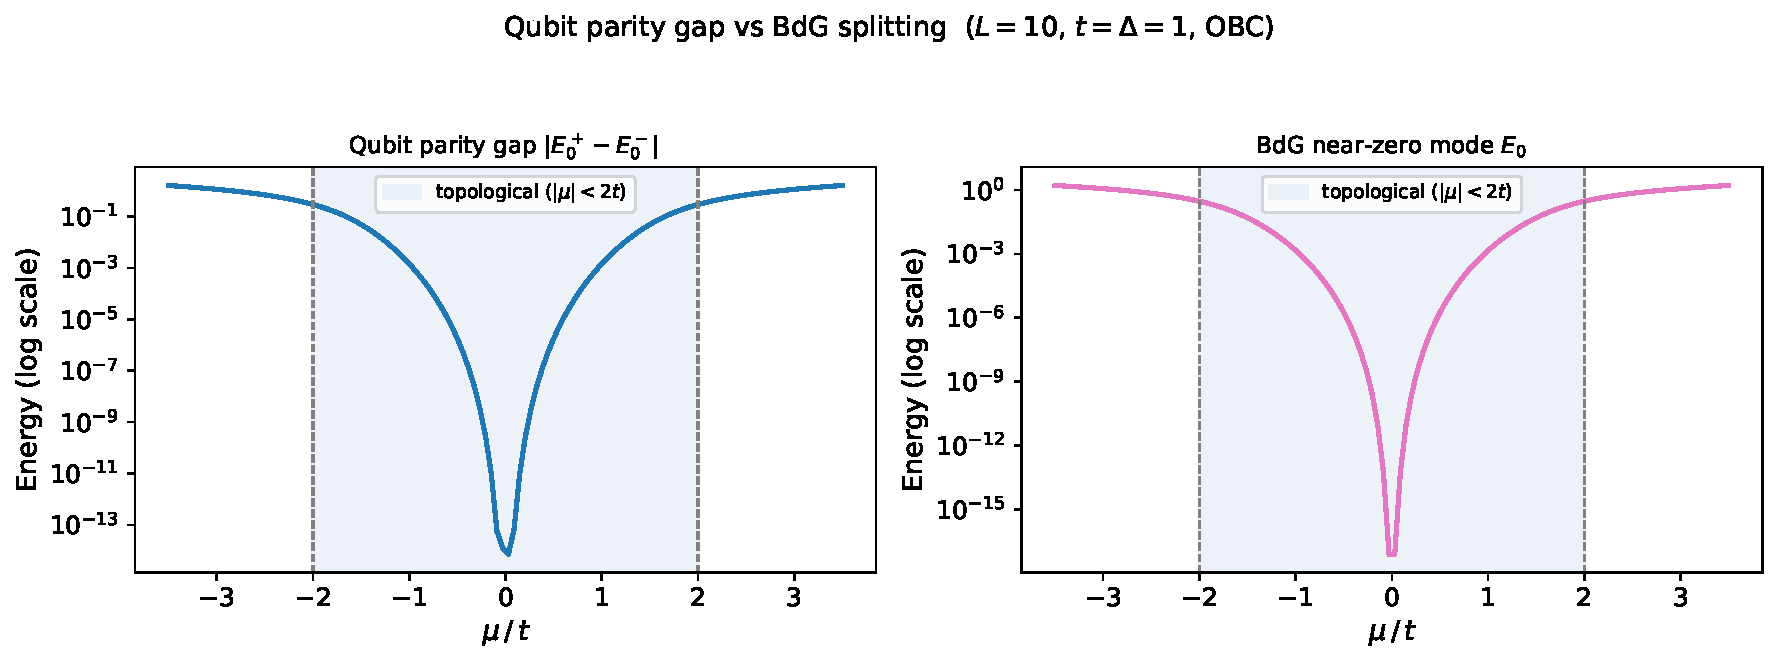
\includegraphics[width=0.9\textwidth]{block2_01_parity_gap_vs_bdg.pdf}
    \caption{Comparison showing the exponential decay of the qubit parity gap (left) perfectly mirroring the BdG near-zero mode splitting (right) within the topological phase ($|\mu| < 2t$).}
    \label{fig:parity_gap}
\end{figure}

The finite-size BdG spectrum operates in a constrained $2L$-dimensional state space, describing single-particle quasiparticle excitations ($\ket{\Psi}$). The lowest positive energy eigenstate in this spectrum, $E_0(L)$, represents the exact energy cost to add one Bogoliubov quasiparticle to the system. As shown in Figure \ref{fig:parity_gap}, in the topological phase, this lowest excitation represents the localized Majorana boundary modes. However, because the left and right Majorana wavefunctions ($\ket{\Psi_L}$ and $\ket{\Psi_R}$) inherently possess exponentially decaying tails, they hybridize on any finite-length chain. The true BdG eigenstates are symmetric and antisymmetric superpositions of these edge modes, possessing a strictly non-zero excitation energy $E_0(L)$.

Conversely, the many-body qubit spectrum evaluates the total collective energy of the system across the entire $2^L$-dimensional many-body Hilbert space ($\ket{\Phi}$). Because the Hamiltonian commutes with the total parity operator, every many-body eigenstate holds a definite parity. The absolute global ground state of the system, $\ket{\Phi_0^{(+)}}$, fundamentally resides in the even-parity sector (analogous to the BCS vacuum), minimizing energy by pairing all fermions.

The lowest odd-parity many-body state, $\ket{\Phi_0^{(-)}}$, is mathematically constructed by acting on the even-parity ground state with the creation operator of the lowest available quasiparticle excitation:
\begin{equation}
    \ket{\Phi_0^{(-)}} = \gamma_0^\dagger \ket{\Phi_0^{(+)}}
\end{equation}
Therefore, the total energy of this odd state is exactly the energy of the even state augmented by the single-particle BdG excitation cost:
\begin{equation}
    E_0^{(-)} = E_0^{(+)} + E_0(L)
\end{equation}

\begin{figure}[h!]
    \centering
    % NOTE TO USER: To ensure this compiles successfully, place the file 'block2_02_qubit_spectrum.pdf' in the same folder as this .tex file.
    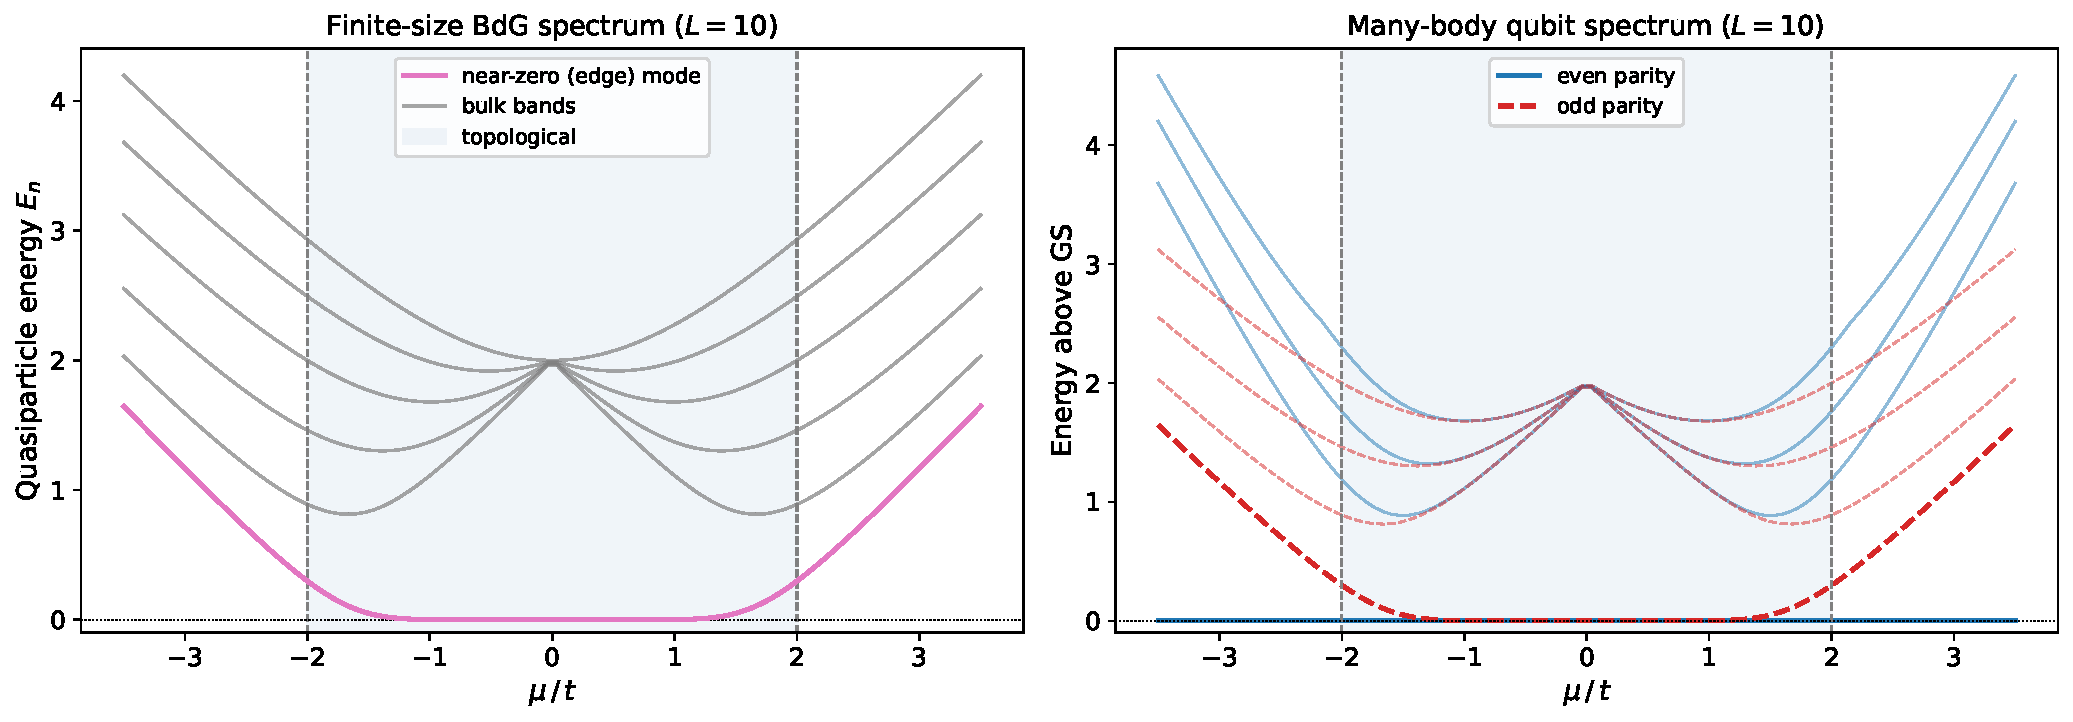
\includegraphics[width=1.0\textwidth]{block2_02_qubit_spectrum.pdf}
    \caption{Side-by-side spectra for $L=10$. The right panel highlights how the many-body even (blue) and odd (red) parity sectors converge into degeneracy exclusively inside the topological phase.}
    \label{fig:qubit_spectrum}
\end{figure}

This fundamental relationship perfectly explains the visual structure of the plotted many-body spectrum in Figure \ref{fig:qubit_spectrum}. Outside the topological phase ($|\mu| > 2t$), injecting a quasiparticle requires breaking a bulk Cooper pair, meaning $E_0(L)$ is macroscopically large. In spectral visualizations, this manifests as a massive energy splitting between the even (blue curves) and odd (red curves) parity sectors. 

Inside the topological phase ($|\mu| < 2t$), the BdG excitation energy $E_0(L)$ corresponds solely to the hybridized Majorana edge modes. As this energy decays exponentially with length $L$, the cost to flip parity drops asymptotically to zero. Consequently, in the many-body spectrum, we observe the complete convergence of the lowest even and odd parity curves. They become perfectly degenerate, visibly illustrating the exactness of the Jordan-Wigner map and manifesting the bulk-boundary correspondence intrinsic to the topological Kitaev chain \cite{Kitaev2001}.

% EMBEDDED BIBLIOGRAPHY
\begin{thebibliography}{9}

\bibitem{Kitaev2001}
A. Y. Kitaev, ``Unpaired Majorana fermions in quantum wires,'' \textit{Physics-Uspekhi}, vol. 44, no. 10S, p. 131, 2001.

\bibitem{JordanWigner1928}
P. Jordan and E. Wigner, ``\"Uber das Paulische \"Aquivalenzverbot,'' \textit{Zeitschrift f\"ur Physik}, vol. 47, no. 9, pp. 631--651, 1928.

\end{thebibliography}

\end{document}
